\documentclass[11pt]{article}
\usepackage{theme}
\usepackage{shortcuts}
\usepackage{mathtools}
% Document parameters
% Document title
\title{Assignment 2 (ML for TS) - MVA 2023/2024}
\author{
Yvann Le Fay \email{yvann.lefay@ensae.fr} \\ % student 1
Antoine Schoonaert \email{antoine.schoonaert@etu.emse.fr} % student 2
}

\DeclarePairedDelimiter\abs{|}{|}

\begin{document}
\maketitle

\section{Introduction}

\paragraph{Objective.} The goal is to better understand the properties of AR and MA processes, and do signal denoising with sparse coding.

\paragraph{Warning and advice.}
\begin{itemize}
    \item Use code from the tutorials as well as from other sources. Do not code yourself well-known procedures (e.g. cross validation or k-means), use an existing implementation.
    \item The associated notebook contains some hints and several helper functions.
    \item Be concise. Answers are not expected to be longer than a few sentences (omitting calculations).
\end{itemize}



\paragraph{Instructions.}
\begin{itemize}
    \item Fill in your names and emails at the top of the document.
    \item Hand in your report (one per pair of students) by Tuesday 5\textsuperscript{th} December 11:59 PM.
    \item Rename your report and notebook as follows:\\ \texttt{FirstnameLastname1\_FirstnameLastname1.pdf} and\\ \texttt{FirstnameLastname2\_FirstnameLastname2.ipynb}.\\
    For instance, \texttt{LaurentOudre\_CharlesTruong.pdf}.
    \item Upload your report (PDF file) and notebook (IPYNB file) using this link: \href{https://docs.google.com/forms/d/e/1FAIpQLSfCqMXSDU9jZJbYUMmeLCXbVeckZYNiDpPl4hRUwcJ2cBHQMw/viewform?usp=sf_link}{docs.google.com/forms/d/e/1FAIpQLSfCqMXSDU9jZJbYUMmeLCXbVeckZYNiDpPl4hRUwcJ2cBHQMw/viewform?usp=sf\_link}.
\end{itemize}


\section{General questions}

A time series $\{y_t\}_t$ is a single realisation of a random process $\{Y_t\}_t$ defined on the probability space $(\Omega, \mathcal{F}, P)$, i.e. $y_t = Y_t(w)$ for a given $w\in\Omega$.
In classical statistics, several independent realisations are often needed to obtain a ``good'' estimate (meaning consistent) of the parameters of the process.
However, thanks to a stationarity hypothesis and a "short-memory" hypothesis, it is still possible to make ``good'' estimates.
The following question illustrates this fact.

\begin{exercise}
An estimator $\hat{\theta}_n$ is consistent if it converges in probability when the number $n$ of samples grows to $\infty$ to the true value $\theta\in\mathbb{R}$ of a parameter, i.e. $\hat{\theta}_n \xrightarrow{\mathcal{D}} \theta$.

\begin{itemize}
    \item Recall the rate of convergence of the sample mean for i.i.d.\ random variables with finite variance.
    \item Let $\{Y_t\}_{t\geq 1}$ a wide-sense stationary process such that $\sum_k |\gamma (k)| < +\infty$.
    Show that the sample mean $\bar{Y}_n = (Y_1+\dots+Y_n)/n$ is consistent and enjoys the same rate of convergence as the i.i.d.\ case. (Hint: bound $\mathbb{E}[(\bar{Y}_n-\mu)^2]$ with the $\gamma (k)$ and recall that convergence in $L_2$ implies convergence in probability.)
\end{itemize}

\end{exercise}

\begin{solution}  % ANSWER HERE
    Let $\{Y_t\}_{t\geq 1}$ be i.i.d random variables with mean $\mu$ and finite variance $\sigma^2$. Let $\bar{Y}_n$ be the sample mean. Tchebychev's inequality states that for any $t>0$
    %
    \begin{equation}
        \mathbb{P}[\abs{\bar{Y}_n- \mu}>t]\leq \frac{\sigma^2}{n t^2},
    \end{equation}
    %
    which goes to $0$ as $n$ goes to $\infty$. Hence, the convergence rate of the sample mean estimator is $O(1/n)$.

    Suppose now that $\{Y_t\}$ is a wide-sense stationary process with $\sum_k \abs{\gamma (k)} < \infty$. We have
    %
    \begin{equation}
        \begin{split}
            \mathbb{E}[(\bar{Y}_n-\mu)^2] & = \frac{1}{n^2} \sum_{1\leq i,j\leq n} \mathbb{E}[(Y_i-\mu) (Y_j-\mu)]\\
            & = \frac{1}{n^2} \sum_{1\leq i,j\leq n} \gamma(\abs{i-j})\\
            & \leq \frac{1}{n^2} \sum_{i=1}^{n}\sum_{k} \abs{\gamma(k)}\\
            & = \frac{1}{n} \sum_{k}\abs{\gamma(k)}  = O(1/n).
        \end{split}
    \end{equation}
    We recover the same convergence rate by Chebychev inequality,
    %
    \begin{equation}
        \mathbb{P}[\abs{\bar{Y}_n-\mu}>t]\leq \frac{\mathbb{E}[(\bar{Y}_n-\mu)^2]}{t^2} = O(1/n).
    \end{equation}
    %
\end{solution}


\newpage
\section{AR and MA processes}

\begin{exercise}[subtitle=Infinite order moving average MA($\infty$)]
Let $\{Y_t\}_{t\geq 0}$ be a random process defined by
\begin{equation}\label{eq:ma-inf}
    Y_t = \varepsilon_t + \psi_1 \varepsilon_{t-1} + \psi_2 \varepsilon_{t-2} + \dots = \sum_{k=0}^{\infty} \psi_k\varepsilon_{t-k}
\end{equation}
where $(\psi_k)_{k\geq0} \subset \mathbb{R}$ ($\psi_0=1$) are square summable, \ie $\sum_k \psi_k^2 < \infty$ and $\{\varepsilon_t\}_t$ is a zero mean white noise of variance $\sigma_\varepsilon^2$.
(Here, the infinite sum of random variables is the limit in $L_2$ of the partial sums.)
\begin{itemize}
    \item Derive $\mathbb{E}(Y_t)$ and $\mathbb{E}(Y_t Y_{t-k})$. Is this process weakly stationary?
    \item Show that the power spectrum of $\{Y_t\}_{t}$ is $S(f) = \sigma_\varepsilon^2 |\phi(e^{-2\pi\iu f})|^2$ where $\phi(z) = \sum_j \psi_j z^j$. (Assume a sampling frequency of 1 Hz.)
\end{itemize}

The process $\{Y_t\}_{t}$ is a moving average of infinite order.
Wold's theorem states that any weakly stationary process can be written as the sum of the deterministic process and a stochastic process which has the form~\eqref{eq:ma-inf}.

\end{exercise}

\begin{solution}  % ANSWER HERE
    Let $t\geq 0$, since $Y_t$ is in $L^2$, $Y_t$ is integrable. We have,
    %
    \begin{equation}
        \mathbb{E}[Y_t] = \lim_{n\to\infty} \mathbb{E}[\sum_{k=0}^{n}\psi_k \varepsilon_{t-k}] = \lim_{n\to\infty} \sum_{k=0}^{n}\psi_k \mathbb{E}[\varepsilon_{t-k}] = 0,
    \end{equation}
    %
    where we use $\mathbb{E}[\varepsilon_k] = 0$ for any $k$.
    Similarly, the square-summable condition on the $\psi_k$'s implies the existence of the second-order moment of $Y_t$ and we can directly work with the infinite sums. Let $0\leq k\leq t$, we have
    %
    \begin{equation}
        \begin{split}
            \mathbb{E}[Y_t Y_{t-k}] &= \mathbb{E}\bigg[\sum_{0\leq j,l<\infty} \psi_j \psi_l \varepsilon_{t-j}\varepsilon_{t-l-k}\bigg]\\
            &= \sum_{0\leq j,l<\infty} \psi_j \psi_l \mathbb{E}[\varepsilon_0 \varepsilon_{j-l-k}]\\
            &=\sigma^2_{\varepsilon} \sum_{l=0}^{\infty} \psi_{l+k}\psi_l<\infty.
        \end{split}
    \end{equation}
    %
    Since the mean and autocovariance functions of the process $Y$ is independent of $t$, $Y$ is stationnary in the wide-sense.
    Let $S$ be defined by $S(f) \coloneqq \sum_{\tau \in \mathbb{Z}} \mathbb{E}[Y_0Y_{\tau}]e^{-2i\pi f \tau}$. Starting from the right-hand side of the equality we are looking to prove, we have (dropping the $\sigma_{\varepsilon}^2$)
    %
    \begin{equation}
        \begin{split}
            \abs{\phi(e^{-2\pi i f})}^2 &= \bigg(\sum_{j=0}^{\infty}e^{-2\pi i f j}\psi_j\bigg)\bigg(\sum_{l=0}^{\infty}e^{2\pi i f l}\psi_l\bigg)\\
            &= \sum_{0\leq j,l<\infty}e^{-2\pi i f (j-l)}\psi_j\psi_l\\
            &= \sum_{\tau\in\mathbb{Z}} \sum_{0\leq j,l<\infty}e^{-2\pi i f \tau}\psi_{j}\psi_{l}\mathds{1}\{j-l=\tau\}\\
            &= \sum_{\tau\in\mathbb{Z}}\sum_{l=0}^{\infty}e^{-2\pi i f \tau}\psi_{\tau + l}\psi_l,
        \end{split}
    \end{equation}
    %
    where going from the first line to the second line is legit because the $\psi_k$'s are square summable. The obtained equation is exactly $S(f)$ up to the multiplicative constant $\sigma_{\varepsilon}^2$. We obtain
    %
    \begin{equation}
        S(f)  = \sigma_{\varepsilon}^2 \abs{\phi(e^{-2\pi i f})}^2.
    \end{equation}
    %

\end{solution}

\begin{exercise}[subtitle=AR(2) process]
Let $\{Y_t\}_{t\geq 1}$ be an AR(2) process, i.e.
\begin{equation}
    Y_t = \phi_1 Y_{t-1} + \phi_2 Y_{t-2} + \varepsilon_t
\end{equation}
with $\phi_1, \phi_2\in\mathbb{R}$.
The associated characteristic polynomial is $\phi(z):=1-\phi_1 z - \phi_2 z^2$.
Assume that $\phi$ has two distinct roots (possibly complex) $r_1$ and $r_2$ such that $|r_i|>1$.
Properties on the roots of this polynomial drive the behaviour of this process.


\begin{itemize}
    \item Express the autocovariance coefficients $\gamma(\tau)$ using the roots $r_1$ and $r_2$.
    \item Figure~\ref{fig:q-ar-2-corr} shows the correlograms of two different AR(2) processes. Can you tell which one has complex roots and which one has real roots?
    \item Express the power spectrum $S(f)$ (assume the sampling frequency is 1 Hz) using $\phi(\cdot)$.
    \item Choose $\phi_1$ and $\phi_2$ such that the characteristic polynomial has two complex conjugate roots of norm $r=1.05$ and phase $\theta=2\pi/6$. Simulate the process $\{Y_t\}_t$ (with $n=2000$) and display the signal and the periodogram (use a smooth estimator) on Figure~\ref{fig:q-ar-2}. What do you observe?
\end{itemize}



\begin{figure}
    \centering
    \begin{minipage}[t]{0.45\textwidth}
    \centerline{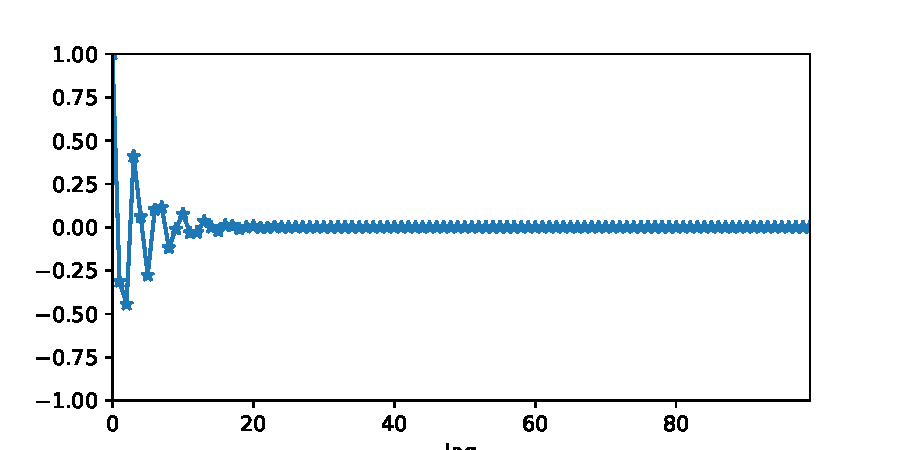
\includegraphics[width=\textwidth]{images/acf1.pdf}}
    \centerline{Correlogram of the first AR(2)}
    \end{minipage}
    \hfill
    \begin{minipage}[t]{0.45\textwidth}    \centerline{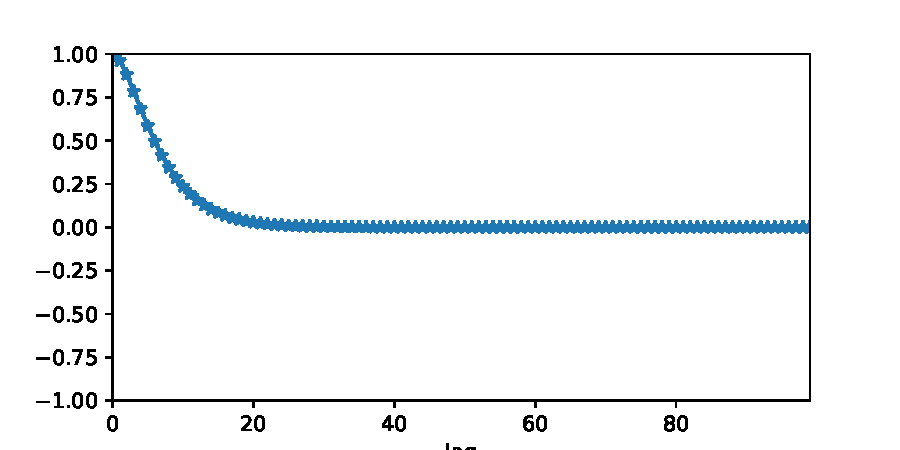
\includegraphics[width=\textwidth]{images/acf2.pdf}}
    \centerline{Correlogram of the second AR(2)}
    \end{minipage}
    \caption{Two AR(2) processes}\label{fig:q-ar-2-corr}
\end{figure}


\end{exercise}

\begin{solution}  % ANSWER HERE
Assuming the process is WSS, multiplying $Y_t$ by $Y_{t+\tau}$ for any $k>0$, and taking the expectation, we obtain for any $\tau$
%
\begin{equation}
    \gamma(\tau)-\phi_1\gamma(\tau-1)-\phi_2\gamma(\tau-2) = 0,
\end{equation}
%
i.e., $\gamma$ is the solution of the second-order recurrent linear equation with characteristic polynomial $P(z) = z^2\phi(1/z) = z^2-\phi_1z-\phi_2$. The roots of $P$ are the inverse of the roots of $\phi$, i.e., $1/r_1$ and $1/r_2$ and since they are distinct, we have for $\abs{\tau}\geq 0$
%
\begin{equation}
\label{eq:cov_ar2}
    \gamma(\tau) = c_1/r_1^\tau  + c_2/r_2^\tau,
\end{equation}
%
for some constants $c_1$ and $c_2$ (determined using the initialisation laws of $Y_0$ and $Y_1$). In the case where $r_1$ has a complex component, i.e., $r_1 = r e^{i \theta}$ for some $r>0$ and $\theta \not\equiv 0 [2\pi]$, we know that $r_2 = \bar{r}_1$ and~\eqref{eq:cov_ar2} becomes
%
\begin{equation}
    \gamma(\tau) = 1/r^\tau (c_1^{'} \cos(\theta \tau) + c_2^{'} \sin(\theta \tau)),
\end{equation}
%
for some constants $c_1'$ and $c_2'$. Otherwise, if $r_1 \in \mathbb{R}$ then $r_2\in \mathbb{R}$. Assuming without loss of generality $\abs{c_1/r_1}>\abs{c_2/r_2}$ with $\abs{r_1}>1$, we see that $\gamma(\tau)\sim c_1 /r_1^{\tau}$ and $\gamma$ displays an exponential decay. We remark that if $r_1<0$, then $\gamma(\tau) \sim c_1/\abs{r_1}^{\tau} (-1)^{\tau}$, hence, we observe an oscillating exponential decay.

Assuming one figure corresponds to the complex case and the other one to the real case, then the left figure corresponds to the complex root case while the right figure correspond to $r_1, r_2\in\mathbb{R}$ with $|r_i|<1$.
\begin{figure}
    \centering
    \begin{minipage}[t]{0.45\textwidth}
    \centerline{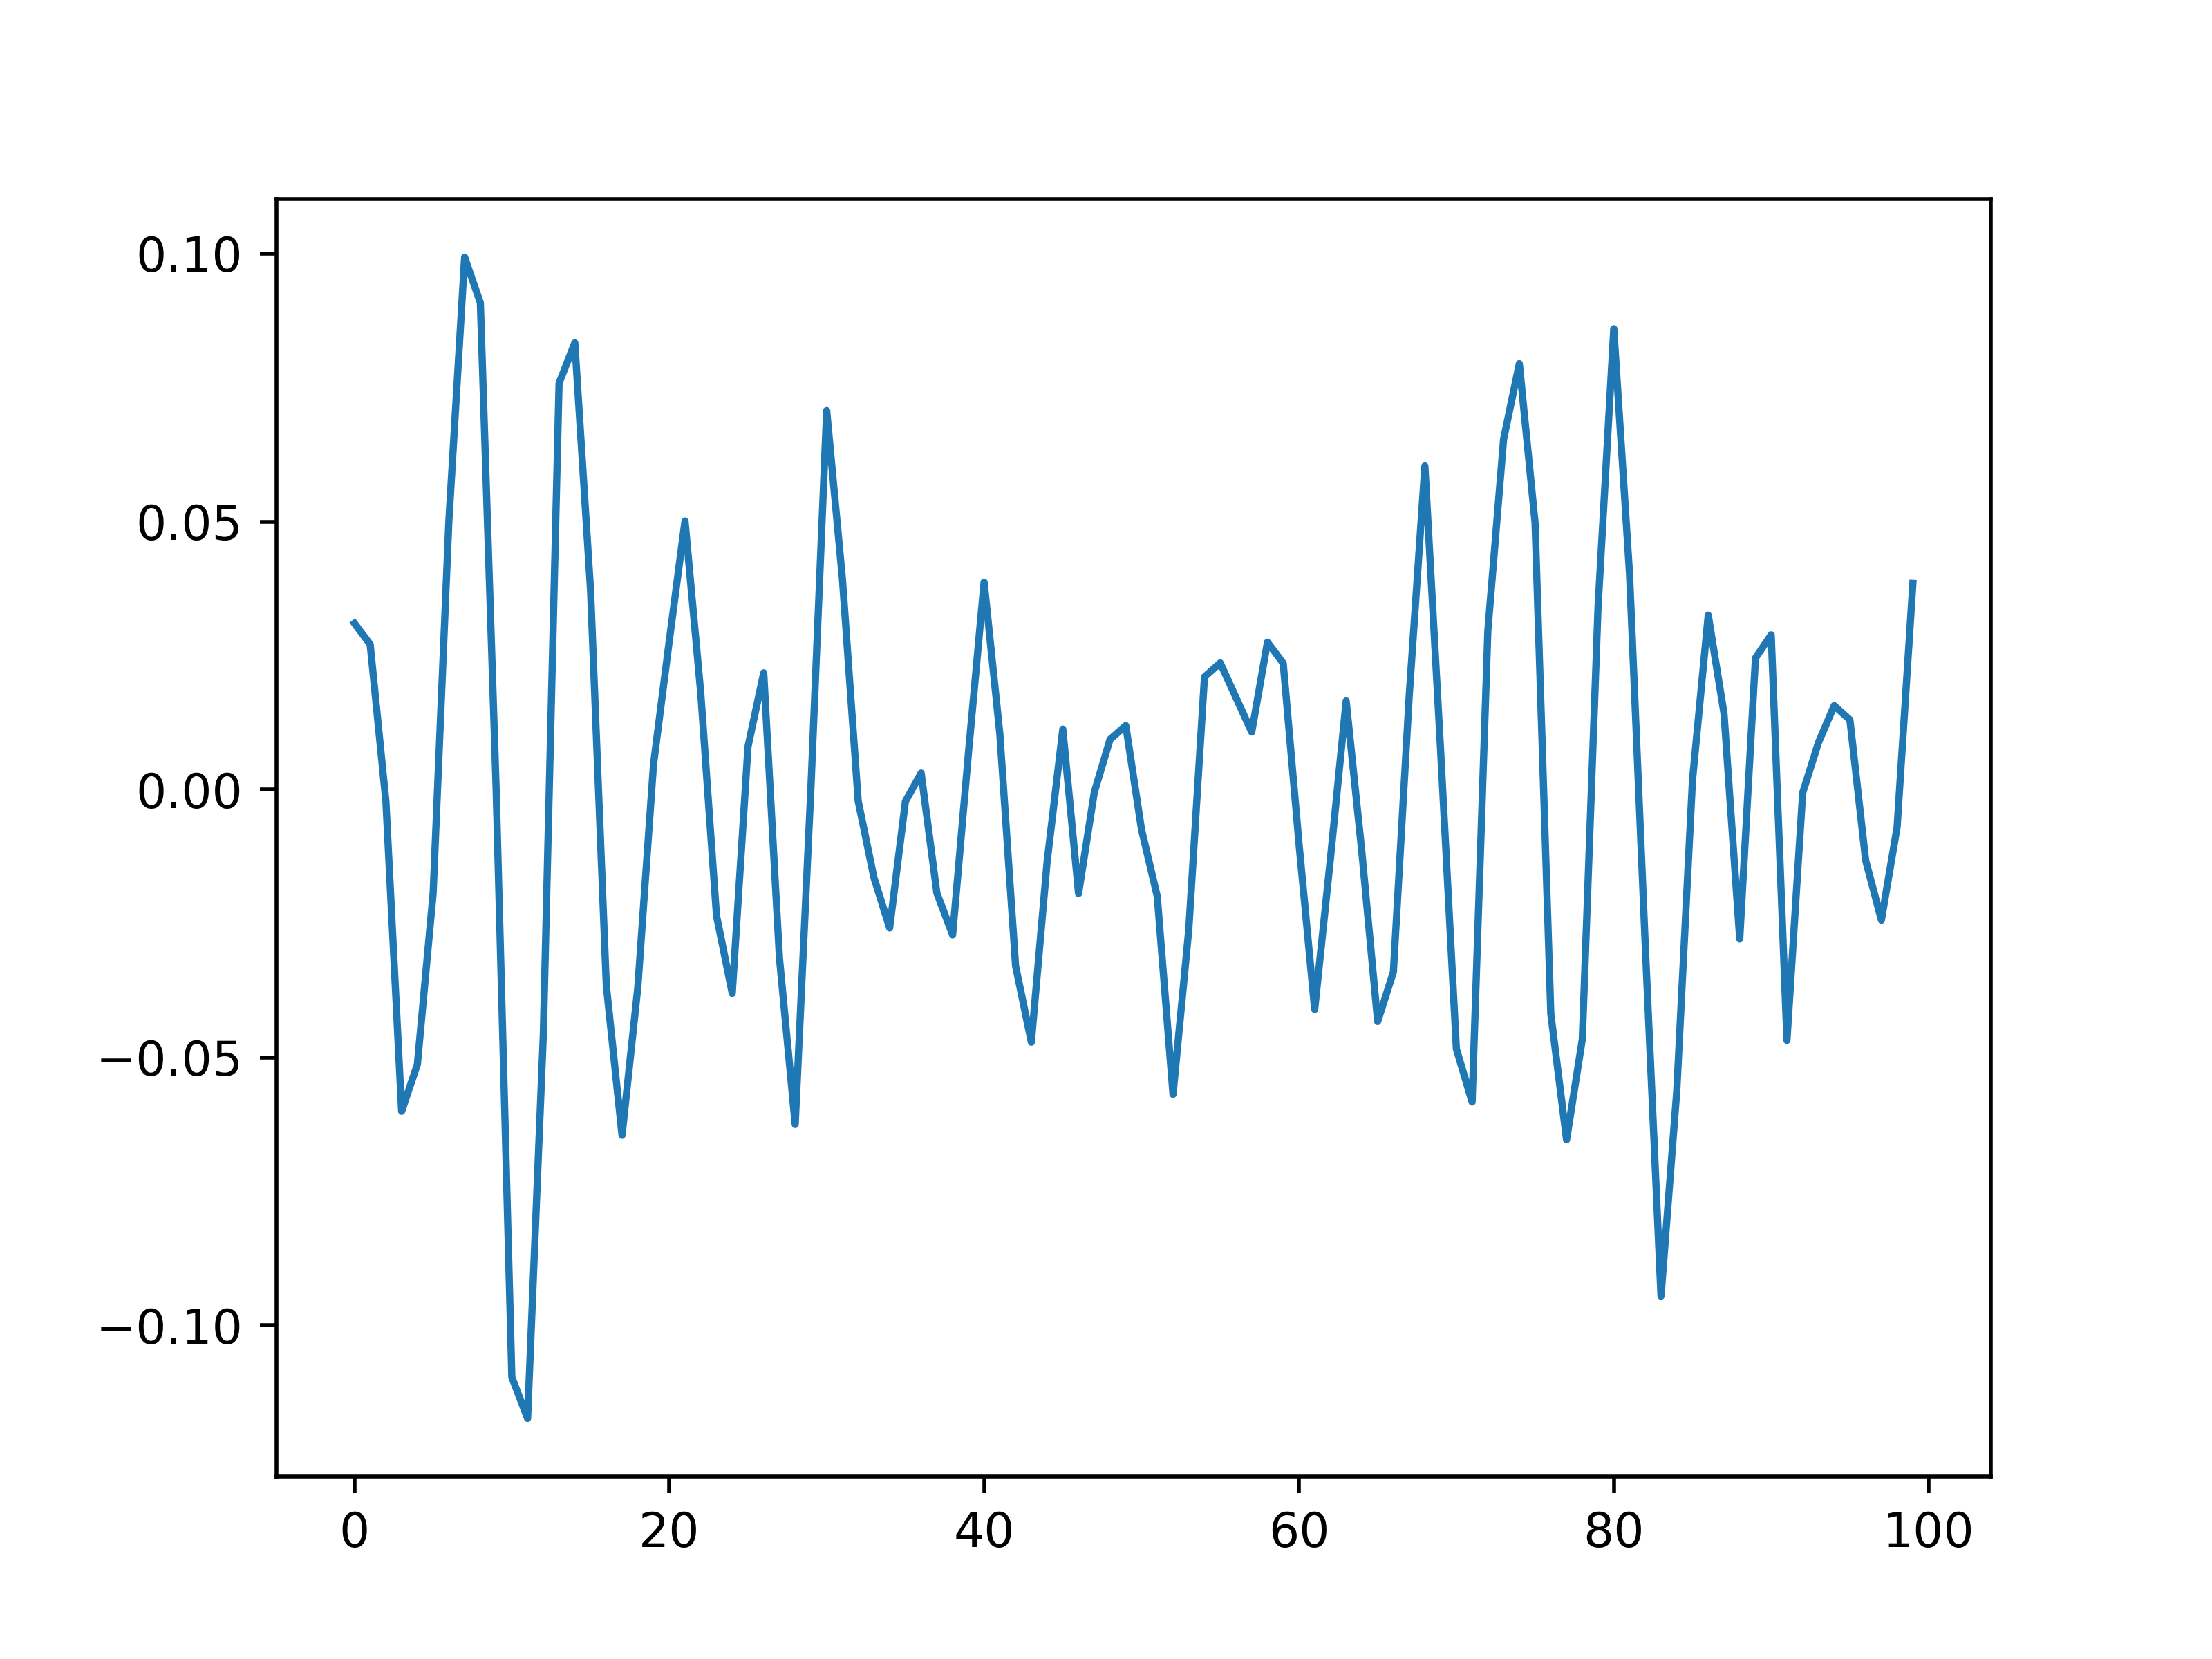
\includegraphics[width=\textwidth]{images/mean_ar_process.png}}
    \centerline{Signal: mean for $1000$ sample paths}
    \end{minipage}
    \hfill
    \begin{minipage}[t]{0.45\textwidth}    \centerline{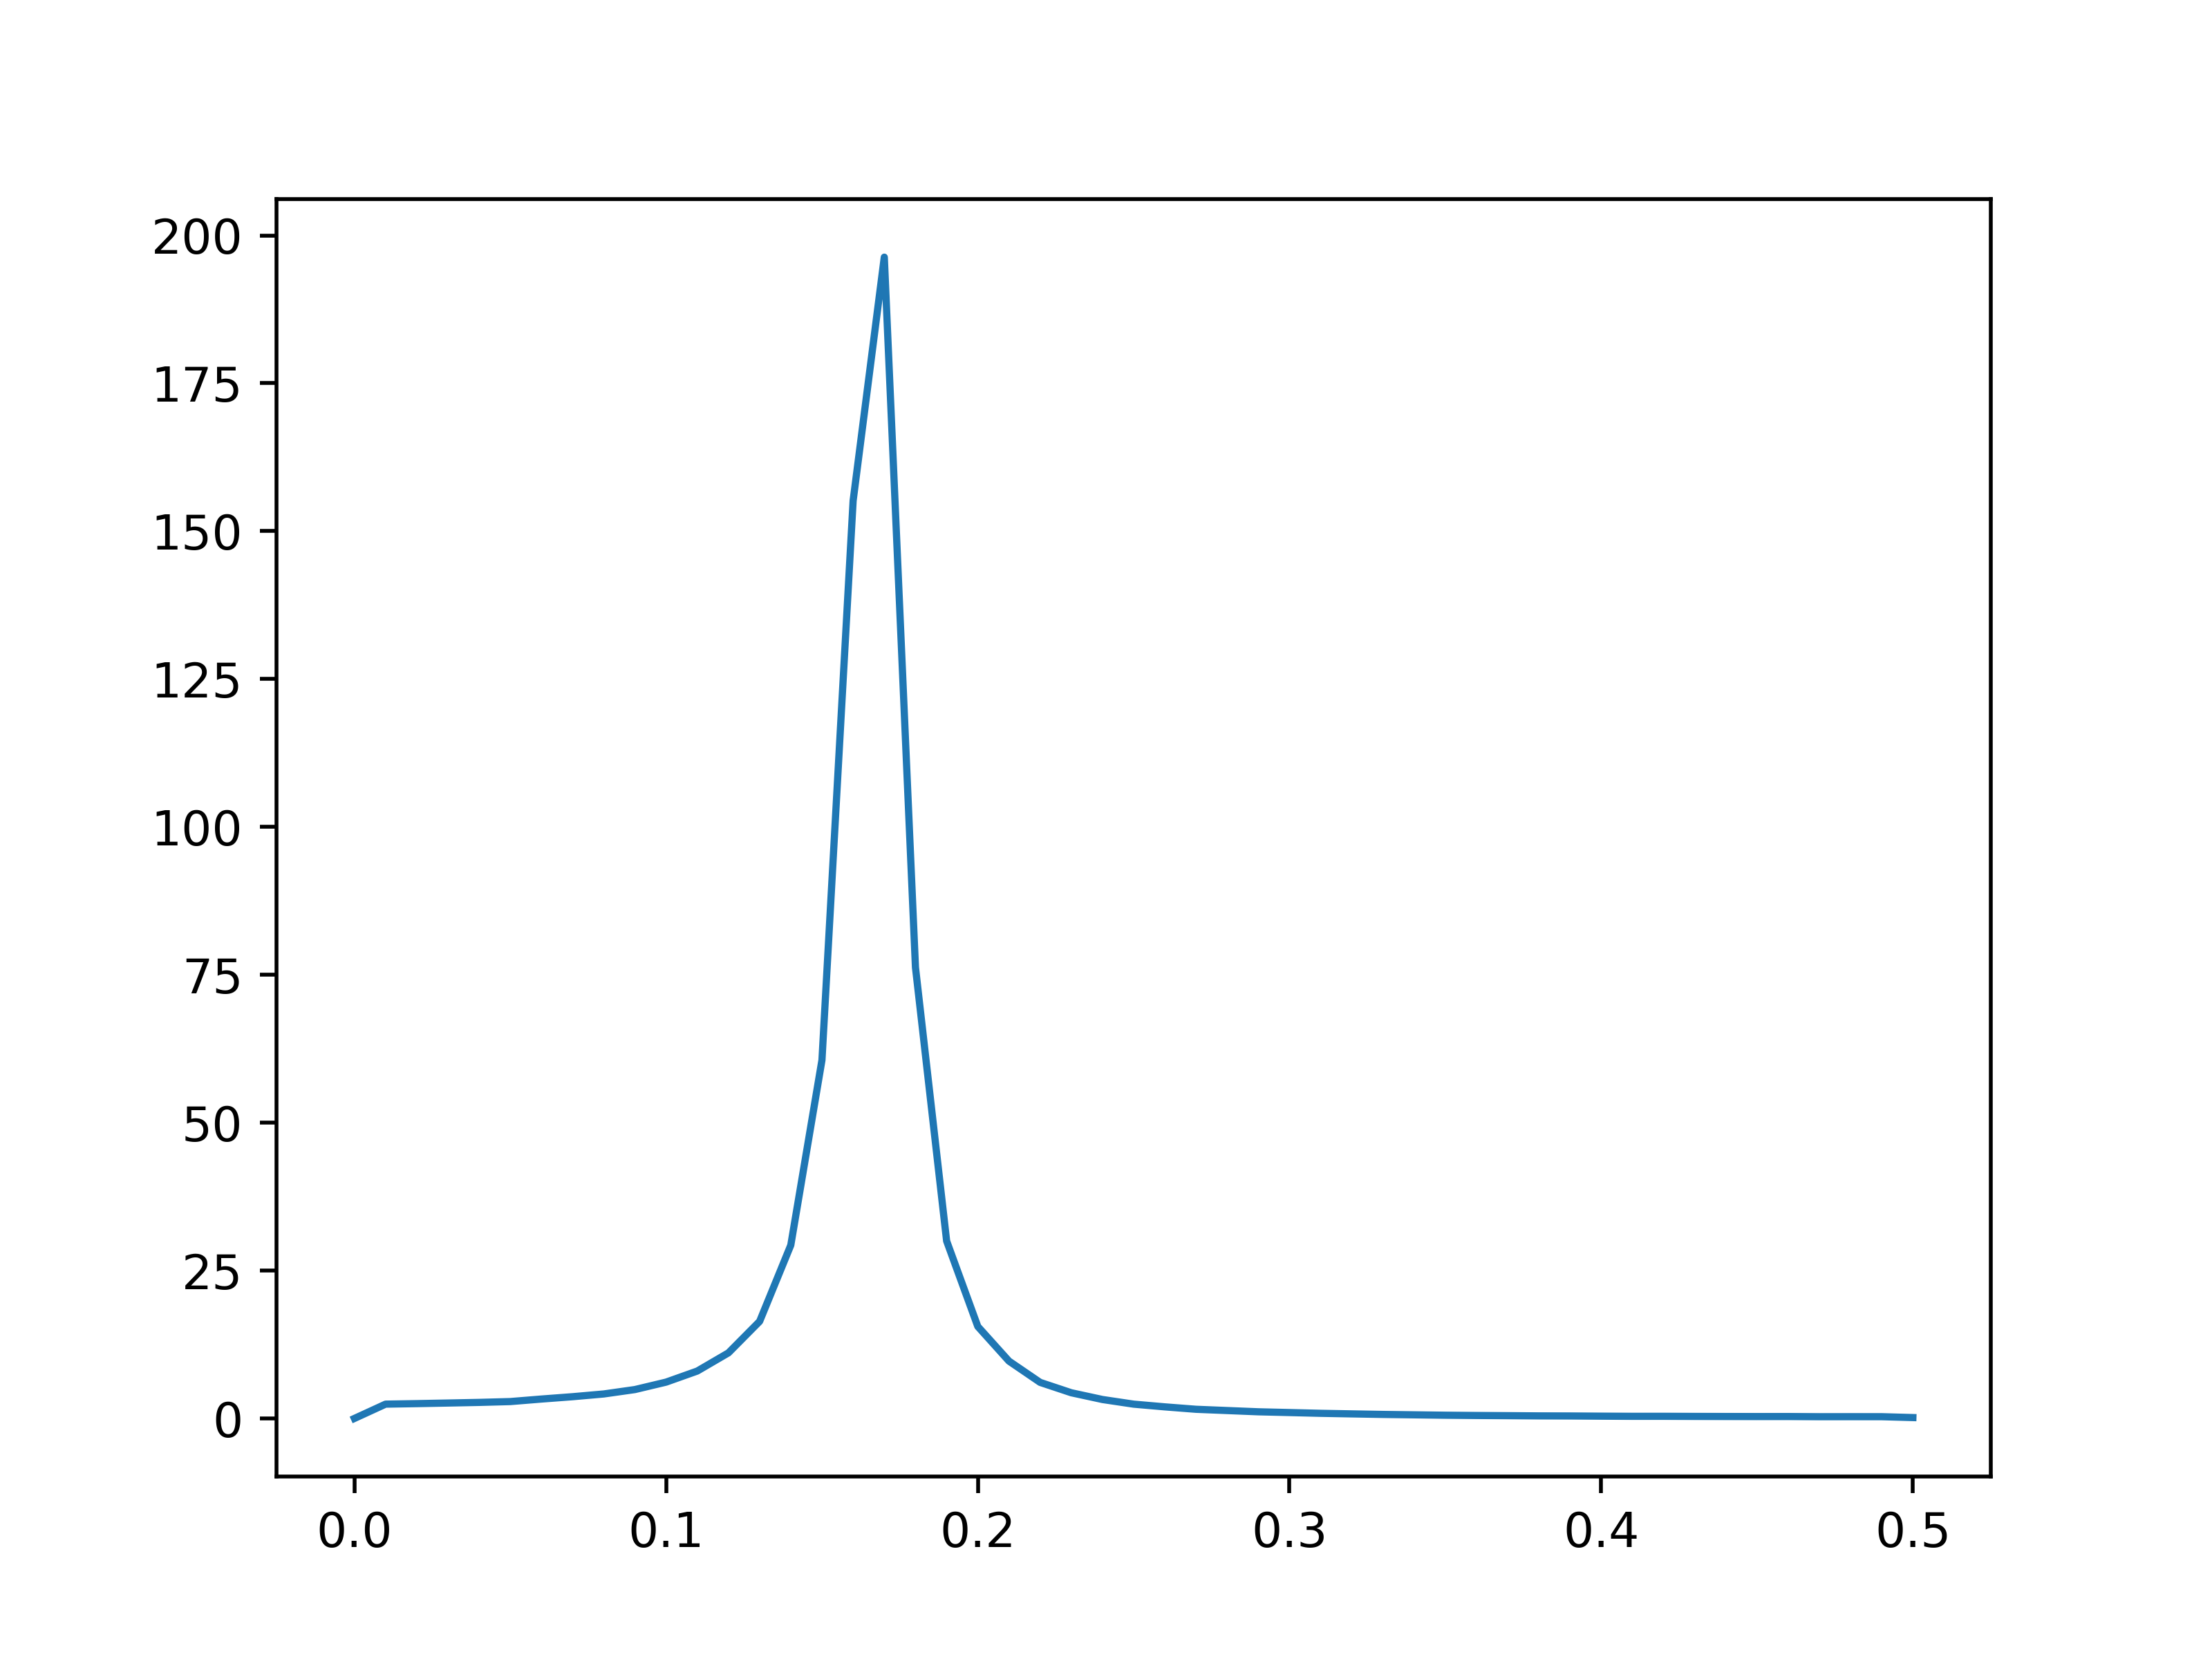
\includegraphics[width=\textwidth]{images/mean_ar_periodogram.png}}
    \centerline{Periodogram: mean for $1000$ sample paths}
    \end{minipage}
    \caption{AR(2) process}\label{fig:q-ar-2}
\end{figure}

Let $t\geq 2$, we have
%
\begin{equation}
    \begin{split}
        Y_t &= \phi_1 Y_{t-1} + \phi_2 Y_{t-2} + \varepsilon_t\\
        &= \phi_1 \varepsilon_{t-1} + (\phi_1^2+\phi_2)Y_{t-2} + \phi_1\phi_2 Y_{t-3} + \varepsilon_{t}\\
        &= \ldots\\
        &= \sum_{j=0}^{t} \varepsilon_{t-j} a_j,
    \end{split}
\end{equation}
%
where we define $a_j$ by
%
\begin{equation}
    a_j = \sum_{l,k\geq 0, l+2k=j}\phi_1^{l}\phi_2^{k}.
\end{equation}
%
We observe that $a_j$ is the $j$-th coefficient of the series $\sum_{j\geq 0} (\phi_1z +\phi_2z^2)^{j}=\frac{1}{1-\phi_1 z -\phi_2 z^2}= \frac{1}{\phi(z)}$.
Thus, using the previous equality for the power-spectrum of a moving-average process, we have
%
\begin{equation}
    S(f) = \sigma_{\varepsilon}^2 \abs{\tilde{\phi}(e^{-2i\pi f})}^2,
\end{equation}
%
where $\tilde{\phi}(z) = \frac{1}{\phi(z)}$, i.e.,
%
\begin{equation}
    S(f) = \frac{\sigma_{\varepsilon}^2}{\abs{\phi(e^{-2i\pi f})}^2}
\end{equation}
%
We have, $z^2P(1/z) = \phi(z)$, with $P(z) = (z-1/r_1)(z-1/r_2)$, hence,
%
\begin{equation}
    \frac{1}{r_1} + \frac{1}{r_2} = \phi_1 \quad -\frac{1}{r_1 r_2} = \phi_2.
\end{equation}
%
We find $\phi_1\approx 0.952$ and $\phi_2 \approx -0.907$.
\end{solution}

\newpage
\section{Sparse coding}

The modulated discrete cosine transform (MDCT) is a signal transformation often used in sound processing applications (for instance to encode a MP3 file).
A MDCT atom $\phi_{L,k}$ is defined for a length 2L and a frequency localisation $k$ ($k=0,\dots,L-1$) by
\begin{equation}
\forall u=0,\dots,2L-1,\quad\phi_{L,k}[u]=w_{L}[u]\sqrt{\frac{2}{L}} \cos [ \frac{\pi}{L} \left(u+ \frac{L+1}{2}\right) (k+\frac{1}{2}) ]
\label{equa_atom}
\end{equation}
where $w_{L}$ is a modulating window given by
\begin{equation}
w_L[u] = \sin \left[{\frac {\pi }{2L}}\left(u+{\frac {1}{2}}\right)\right].
\end{equation}


\begin{exercise}[subtitle=Sparse coding with OMP]
For the signal provided in the notebook, learn a sparse representation with MDCT atoms.
The dictionary is defined as the concatenation of all shifted MDCDT atoms for scales $L$ in $[32, 64, 128, 256, 512, 1024]$.

\begin{itemize}
    \item For the sparse coding, implement the Orthogonal Matching Pursuit (OMP). (Use convolutions to compute the correlations coefficients.)
    \item Display the norm of the successive residuals and the reconstructed signal with 10 atoms.
\end{itemize}

 \end{exercise}
\begin{solution}

The aim of this exercise is to re-create a signal from atoms defined by \ref{equa_atom}.

Firstly, we implement the creation of the dictionary with normalisation.

Secondly, we implement the Orthogonal Matching Pursuit using convolution to calculate the correlation coefficients. At each stage, we calculate the convolution between the residual signal and each atom, so the correlation coefficient corresponds to the maximum of the convolution result. The new atom to be added is the one with the highest coefficient. In doing this, the only atoms taken were those of length 2048 because, since they are longer, the convolution has a greater maximum. So we decided to divide each coefficient obtained by a value proportional to the size of the atom. The value corresponds to the average (over atoms of the same length) of the maximum values of the convolution. It is by doing this that we obtain the best reconstruction.

Figure \ref{q4} shows our results. We are aware that there is still room for improvement. We can see a peak at around 750, due to the end of an atom. This appears when we "force" the acceptance of small frequencies by dividing the coefficients as explained above. The visual aspect is very bad at this point but thanks to this the final norm of the residue decreased from 21 to 18.





\begin{figure}
    \centering
    \begin{minipage}[t]{1\textwidth}
    \centerline{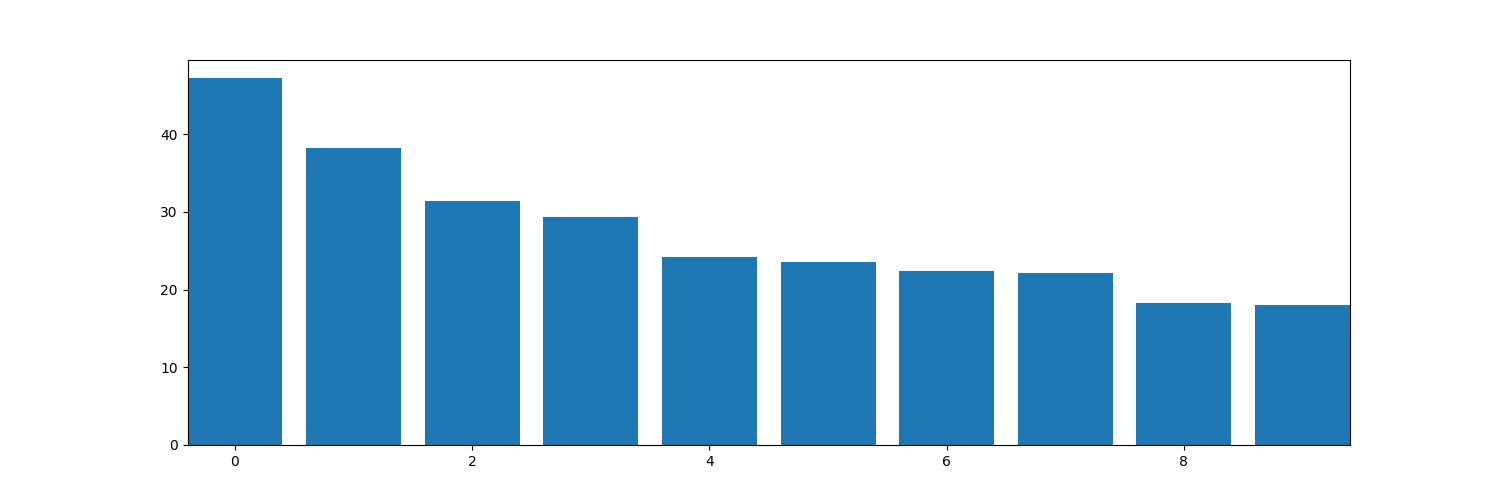
\includegraphics[width=\textwidth]{images/residu.png}}
    \centerline{Norms of the successive residuals}
    \end{minipage}
    \hfill
    \begin{minipage}[t]{1\textwidth}    \centerline{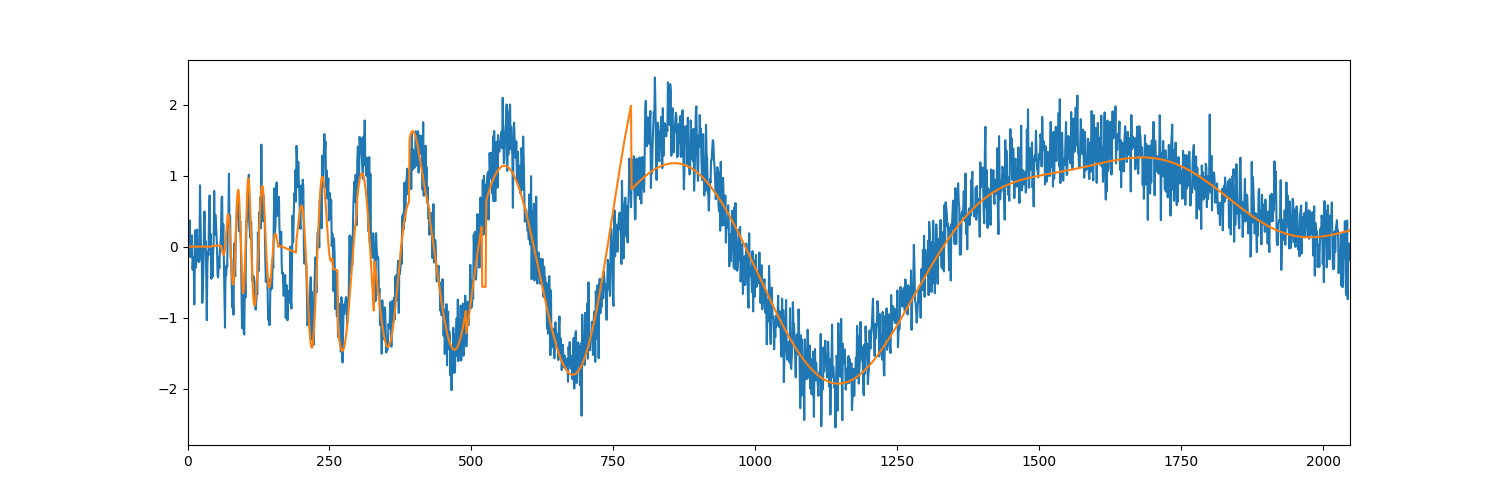
\includegraphics[width=\textwidth]{images/signal_reconstruit.png}}
    \centerline{Reconstruction with 10 atoms}
    \end{minipage}
    \caption{Question 4}
    \label{q4}
\end{figure}





\end{solution}

\end{document}